\chapter{Data in Tao}
\label{c:data}
\index{Data|hyperbf}

The term \vn{``data''} denotes anything that can be calculated by
\tao. This includes the vertical orbit at a particular position or the
horizontal emittance of a storage ring. Data can be plotted or used in
lattice correction and design (\sref{c:opti}). This chapter explains
how data is organized in \tao while Section~\sref{s:init.data}
explains how to define the structures that hold the data in the
initialization files. When running \tao, the \vn{show data}
(\sref{s:show}) command can be used to view information about the
data.


%------------------------------------------------------------------------
\section{Data Organization}
\label{s:data.org}

\begin{figure}
  \centering
  \includegraphics[width=4in]{data-tree.eps}
  \caption[Data tree structure]
{A \vn{d2\_data} structure holds a set of \vn{d1\_data} structures. 
A \vn{d1\_data} structure holds an array of datums.}
  \label{f:data.tree}
\end{figure}

\index{d2_data}\index{d1_data}
The horizontal orbit at a particular BPM is an example of an
individual \vn{datum}.  For ease of manipulation, arrays of datums are
grouped into what is called a \vn{d1_data} structure. Furthermore,
sets of \vn{d1_data} structures are grouped into what is called a
\vn{d2_data} structure.  This is illustrated in
Figure~\ref{f:data.tree}.  For example, a \vn{d2_data} structure for
orbit data could contain two \vn{d1_data} structures --- one
\vn{d1_data} structure for the horizontal orbit data and another
\vn{d1_data} structure for the vertical orbit data. Each datum of,
say, the horizontal orbit \vn{d1_data} structure would then correspond
to the horizontal orbit at some point in the machine.

When issuing \tao commands, all the
data associated with a \vn{d2_data} structure is specified using the
\vn{d2_data} structure's \vn{name}.  The data associated with a
\vn{d1_data} structure is specified using the format
\begin{example}
  d2_name.d1_name
\end{example}
For example, if a \vn{d2_data} structure has the
name ``\vn{orbit}'', and one of its \vn{d1_data} structures has the
name ``\vn{x}'', then \tao commands that refer to the data in this
\vn{d1_data} structure use the name ``\vn{orbit.x}''. Sometimes there
is only one \vn{d1_data} structure for a given \vn{d2_data}
structure. In this case the data can be referred to simply by using
the \vn{d2_data} structure's name. The individual datums can be
referred to using the notation
\begin{example}
  <d2_name>.<d1_name>[<list_of_datum_indexes>]
\end{example}
For example, \vn{orbit.x[10]} refers to the horizontal orbit datum
with index 10. Notice that the beginning (lowest) datum index is user
selectable and is therefore not necessarily 1. 

It is important to note that the name given to \vn{d2_data} and \vn{d1_data}
structures is arbitrary and does not have to correspond to the 
type of data contained in the 
structures. In fact, a \vn{d1_data} array can contain hetogeneous data types.
Thus, for example, it is perfectly permissible (but definitely not recommended) 
to set up the data structures so that, say, \vn{orbit.x[10]} 
is the $a$-mode emittance at a certain element and \vn{orbit.x[11]}
is the $b$-mode beta function at the same element.

Ranges of data can be referred to using using a comma \vn{,} to
separate the indexes combined with the notation \vn{n1:n2} to specify
all the datums between \vn{n1} and \vn{n2} inclusive. For example
\begin{example}
  orbit.x[3:6,23]
\end{example}
refers to datums 3, 4, 5, 6, and 23. 

If multiple universes are present, then, as explained in
\sref{s:universe}, the prefix \vn{"@"} may be used to specify which
universe the data applies to. The general notation is
\begin{example}
  [<universe_range>]@<d2_name>.<d1_name>[<datum_index>]
\end{example}
Examples:
\begin{example}
  [2:4,7]@orbit.x ! The \vn{orbit.x} data in universes 2, 3, 4 and 7.
  [2]@orbit.x     ! The \vn{orbit.x} data in universe 2. 
  2@orbit.x       ! Same as "2@orbit.x".
  orbit.x         ! The \vn{orbit.x} data in the current viewed universe.
  -1@orbit.x      ! Same as "orbit.x".
\end{example}

As explained in Section~\sref{s:data.anatomy}, each individual datum
has a number of components. The syntax to refer to a component is:
\begin{example}
  d2_name.d1_name[datum_index]|component
\end{example}
For example:
\begin{example}
  orbit.x[3:10]|meas     ! The measured data values
\end{example}

In referring to datums, a ``\vn{*}'' can be used as a wild card to 
denote ``all''. Thus:
\begin{example}
  *@orbit.x       ! The \vn{orbit.x} data in all universes.
  *               ! All the data in the currently viewed universe.
  *.*             ! Same as "*"
  *@*             ! All the data in all the universes. 
  *@*.*           ! Same as "*@*"
  orbit.x[*]|meas ! All measured values of orbit.x
  orbit.x[]|meas  ! No values. That is, the empty set.
  orbit.x|meas    ! Same as orbit.x[*]|meas.
\end{example}
The last example shows that when referring to an entire block of data
encompassed by a \vn{d1_data} structure, the \vn{[*]} can be omitted.

%------------------------------------------------------------------------
\section{Anatomy of a Datum}
\label{s:data.anatomy}

Each datum has a number of quantities associated with it:
\begin{example}
  data_type        ! Character: Type of data: "orbit.x", etc.
  ele_name         ! Character: Name of lattice element where datum is evaluated.
  ele_start_name   ! Character: Name of starting lattice element in a range.
  ele_ref_name     ! Character: Name of reference lattice element.
  merit_type       ! Character: Type of constraint: "target", "max", etc.
  data_source      ! Character: How the datum is calculated. "lattice", or "beam".
  ix_ele           ! Integer: Index of "ele" in the lattice element list.
  ix_ele_start     ! Integer: Index of "ele_start" in the lattice element list.
  ix_ele_ref       ! Integer: Index of "ele_ref" in the lattice element list.
  ix_ele_merit     ! Integer: Lattice index where merit is evaluated.
  ix_d1            ! Integer: Index number in d1_data structure
  ix_data          ! Integer: Index in the global data array
  ix_dModel        ! Integer: Row number in the dModel_dVar derivative matrix.
  ix_bunch         ! Integer: Bunch number to get the data from.
  meas             ! Real: Measured datum value. 
  ref              ! Real: Measured datum value from the reference data set.
  model            ! Real: Datum value as calculated from the model.
  design           ! Real: What the datum value is in the design lattice.
  old              ! Real: The model at some previous time.
  base             ! Real: The value as calculated from the base model.
  fit              ! Real: The value as calculated from a fitting procedure.
  invalid          ! Real: The value used for delta_merit if good_model = False.
  delta_merit      ! Real: Diff used to calculate the merit function term 
  weight           ! Real: Weight for the merit function term
  merit            ! Real: Merit function term value: weight * delta^2
  s                ! Real: longitudinal position of ele.
  exists           ! Logical: Does the datum exist?
  good_model       ! Logical: Does the model  component contain a valid value?
  good_design      ! Logical: Does the design component contain a valid value?
  good_base        ! Logical: Does the base   component contain a valid value?
  good_meas        ! Logical: Does the meas   component contain a valid value?
  good_ref         ! Logical: Does the ref    component contain a valid value?
  good_user        ! Logical: Does the user want this datum used in optimization?
  good_opt         ! Logical: Can be used in Tao extensions.
  good_plot        ! Logical: Can be used in Tao extensions.
  useit_plot       ! Logical: Is this datum to be used in plotting?
  useit_opt        ! Logical: Is this datum to be used for optimization?
\end{example}
When running \tao, the \vn{show data}
(\sref{s:show}) command can be used to view the components of a datum. 
The \vn{set} command (\sref{s:set}) can be used to set some of these components.

%------------------------------------------------------------------------
\section{Datum values}
\label{s:datum.values}

\index{Data!measured}\index{Data!reference}\index{Data!model}
\index{Data!base}\index{Data!design}
A given datum has six values associated it:
\vspace{-2ex}
\begin{description}
  \vspace{-1ex}
  \item[meas] \Newline 
The value of the datum as obtained from some measurement. This is the
target or limit value that is used when running the optimizer. When
doing lattice design, the measured value corresponds to a constraint
value (\ref{c:opti}).
  \vspace{-1ex}
  \item[ref] \Newline
The reference datum value as obtained from some reference measurement. For example,
a measurement before some variable is varied could be designated as
the \vn{reference}, and the datum taken after the variation could be 
designated the \vn{measured} datum.
  \vspace{-0.5ex}
  \item[model] \Newline
The value of the datum as calculated from the \vn{model} lattice (\sref{s:lattice}).
  \vspace{-0.5ex}
  \item[design] \Newline
The value of the datum as calculated from the \vn{design} lattice (\sref{s:lattice}).
  \vspace{-0.5ex}
  \item[base] \Newline
The datum value as calculated from the \vn{base} lattice (\sref{s:lattice}).
  \vspace{-0.5ex}
  \item[old] \Newline
A datum value that was saved at some point in \tao's calculations. This value
can be ignored.
\end{description}

%------------------------------------------------------------------------
\section{Datums in Optimization}
\label{s:datum.opt}

When using optimization for lattice correction or lattice design
(\sref{c:opti}), Individual datums can be excluded from the process
using the \vn{veto} (\sref{s:veto}), \vn{restore} (\sref{s:restore}),
and \vn{use} (\sref{s:use}) commands. These set the \vn{good_user}
component of a datum. This, combined with the setting \vn{exists},
\vn{good_meas}, \vn{good_ref}, and \vn{good_opt}
determine the setting of \vn{useit_opt} which is the component that
determines if the datum is used in the computation of the merit
function. The settings of everything but \vn{good_user} is determined
by \tao

The \vn{exists} component is set by \tao to True if the datum exists
and False otherwise. A datum may not exist if the type of datum
requires the designation of an associated element but the
\vn{ele_name} component is blank. For example, a \vn{d1_data} array
set up to hold orbit data may use a numbering scheme that fits the
lattice so that , say, datum number 34 in the array does not
correspond to an existing BPM.

The \vn{good_model} component is set according to whether a datum
value can be computed from the \vn{model} lattice. For example, If a
circular lattice is unstable, the beta function and the closed orbit
cannot be computed. Similarly, the \vn{good_design} and \vn{good_base}
components mark whether the \vn{design} and \vn{base} values
respectively are valid.

When doing optimization, the \vn{delta_merit} component is set to the
\vn{delta} value used in computing the contribution to the merit
function (\sref{s:generalized.design}). If the datum's value cannot be
computed, that is, \vn{good_model} is False, or, if the design or base
values are being used in the merit calculation, \vn{good_base} or
\vn{good_design} is False, then the \vn{invalid} component is used for
\vn{delta_merit}.

\vn{good_meas} is set True if the \vn{meas} component value is set in
the data initialization file (\sref{s:init.data}) or is set using the
\vn{set} command (\sref{s:set}). Similarly, \vn{good_ref} is set True
if the \vn{ref} component has been set. \vn{good_ref} only affects the
setting of \vn{useit_opt} if the optimization is using reference data
as set by the global variable \vn{opt_with_ref} (\sref{s:globals}).

Finally \vn{good_opt} is meant for use in custom versions of \tao
(\sref{c:custom.tao}) and is always left True by the standard \tao code.

Example of using a \vn{show data} (\sref{s:show}) to check the logicals
in a datum:
\begin{example}
  Tao> show data 3@beta[1]

  Universe:   3
  %ele_name          = IP_L0
  %ele_ref_name      =
  %ele_start_name    =
  %data_type         = beta.a
      ... etc ...
  %exists            =  T
  %good_model        =  T
  %good_meas         =  F
  %good_ref          =  F
  %good_user         =  T
  %good_opt          =  T
  %good_plot         =  F
  %useit_plot        =  F
  %useit_opt         =  F
\end{example}
Here \vn{useit_opt} is False since \vn{good_meas} is False and
\vn{good_meas} is False since the \vn{meas} value of the datum (not
shown) was not set in the \tao initialization file.

%------------------------------------------------------------------------
\section{Tao Data Types}\index{Data!Data Types}
\label{s:data.types}

Data can be classified by how it is calculated. This is set by the
\vn{data_source} parameter associated with an attribute. If the data
comes from particle beam tracking, \vn{data_source} must be set to
\vn{"beam"}. For everything else, \vn{data_source} must be set to
\vn{"lattice"}. Some datum types, like the floor position of an
element, only make sense with a \vn{"lattice"} \vn{data_source}. Other
types, like \vn{dpx_dx}, only make sense with a \vn{"beam"}
\vn{data_source}. There is a third class of data types, like
\vn{emit.a} that can take a \vn{"lattice"} or \vn{"beam"}
\vn{data_source}. It is important to keep in mind that with this third
case, such datums will have a different value depending upon what
\vn{data_source} is used.  Table~\ref{t:data.beam} lists the
predefined data types in \tao that are valid for a \vn{"beam"}
\vn{data_source} (\sref{s:init.data}) and
Table~\ref{t:data.lattice} lists the predefined data types in
\tao that are valid for a \vn{"lattice"} \vn{data_source}.

It is important to note the difference between the \vn{d2.d1} name
that is used to refer to a given set of data and the actual type of
the data of the datums in the set. The \vn{d2.d1} name is arbitrary
and is specified in the \tao initialization file
(\sref{s:init.data}). Often, these names do reflect the actual type of
data. However, there is no mandated relationship between the two. For example,
it is perfectly possible to set create a data set with a \vn{d2.d1}
name of \vn{orbit.x} to hold, say, global floor position data. In
fact, the datums in a given \vn{d1} array do not all have to be of the
same type. Thus the user is free to group data as s/he sees fit.

Associated with a datum are three lattice elements called the
\vn{evaluation element}, the \vn{reference element}, and the
\vn{start element}. The corresponding components in a datum are
shown in Table~\ref{t:datum.elements}.
These three elements may be specified for a datum by either setting
the name component or the index component of the datum. Using the
element index over the element name is necessary when more than one
element in the lattice has the same name.

\begin{table}[htb]
\centering
\begin{tabular}{lll}
  \toprule
  &\multicolumn{2}{c}{\it Data Component} \\ \cmidrule{2-3}
  {\it Element} & {\it name} & {\it index} \\ \midrule
  Reference Element  & \vn{ele_ref_name}   & \vn{ix_ele_ref}   \\
  Start Element      & \vn{ele_start_name} & \vn{ix_ele_start} \\
  Evaluation Element & \vn{ele_name}       & \vn{ix_ele}       \\ \bottomrule
\end{tabular}
\caption{The three lattice elements associated with a datum may be
specified in the datum by setting the appropriate name component or by 
setting the appropriate index component.}
\label{t:datum.elements}
\end{table}

Some datums, like the emittance in a circular ring, do not have
associated lattice elements and their corresponding element names will
be blank. All other datums must have an associated evaluation element
that is specifed by setting the \vn{ele_name} or \vn{ix_ele} datum
component. If a datum has an associated evaluation element, but no
associated start or reference elements, the \vn{model} value of that
datum is the value of the \vn{data_type} at the evaluation
element. For example, if a datum has:
\begin{example}
  data_type      = "orbit.x"
  ele_name       = "q12"
\end{example}
then the \vn{model} value of this datum will be the horizontal orbit
at the element with name \vn{q12}.

If a datum has an associated start element, specified by either
setting the \vn{ele_start_name} or \vn{ix_ele_start} datum components, the
datum is evaluated over a region from the exit end of the start element
to the exit end of evaluation element. For example, if a datum has:
\begin{example}
  data_type      = "beta.a"
  ele_name       = "q12"
  ele_start_name = "q45"
  merit_type     = "max"
\end{example}
then the \vn{model} value of this datum will be the maximum value of the a-mode
beta function in the region from the exit end of the element with name
\vn{q12} to the exit end of the element with name \vn{q45}. Notice
that when a range of elements is used, a \vn{merit_type} of
\vn{target} does not make sense.

If a datum has an associated reference element, specified by either
setting the \vn{ele_ref_name} or \vn{ix_ele_ref} datum components, the
\vn{model} value of the datum is the value at the evaluation element (or the value
over the range \vn{ele_start} to the evaluation element if \vn{ele_start} is
specified), minus the \vn{model} value at \vn{ele_ref}. For example,
if a datum has:
\begin{example}
  data_type      = "beta.a"
  ele_name       = "q12"
  ele_start_name = "q45"
  ele_ref_name   = "q1"
  merit_type     = "max"
\end{example}
then the \vn{model} value of the datum will be the same as the
previous example minus the value of the a-mode beta function at the
exit end of element \vn{q1}. There are a number of exceptions to the
above rule and datum types treat the reference element in a different
manner. For example, the \vn{r.} data type uses the reference element
as the starting point in constructing a transfer matrix.

The individual data types are described below:

  \begin{description}
  \index{beta.}
  \item[beta.] \Newline
\vn{beta.a} and \vn{beta.b} are the lattice beta functions. \vn{beta.x} and
\vn{beta.y} are beam projected beta functions defined by
\begin{equation}
  \beta.x = \frac{<x^{2}>}{\sqrt{<x^{2}> <x'^{2}> - <x x'>^{2}}}.
\end{equation}
where the average \vn{<>} is over all the particles in the beam.

Note: If the beta function is calculated from the beam distribution,
the emittance must be non-zero.

  \index{emit.}
  \item[emit.] \Newline
Emittance can be calculated in one of two ways. One way is to
calculate it from a tracked beam. The other is from the lattice using
the standard radiation integrals (see the Bmad manual). For a linear
lattice, the emittance varies along the length of the line while for a
circular lattice there is a single emittance number. \vn{emit.a}
and \vn{emit.b} are the standard normal mode emittances. With
beam tracking, there are also \vn{projected emittances} which give an
indication of what the beam looks like if projected onto the $x$ or
$y$ axes:
\begin{equation}
  \mbox{emit.x} \equiv \sqrt{<x^2> <p_x^2> - <x p_x>^2}
\end{equation}
Notice that this does {\emph not} correspond to the standard emittance
definition in one dimension:
\begin{equation}
  \epsilon_x = \sqrt{<(x - \eta_x \, p_z)^2> <(p_x - \eta'_x \, p_z)^2> - 
  <(x - \eta_x \, p_z) \, (p_x - \eta'_x \, p_z)>^2}
\end{equation}
\vn{emit.x} and \vn{emit.y} are the projected emittances.
Also notice that the projected emittance is sometimes defined using
$x'$ and $y'$ in place of $p_x$ and $p_y$. However, in the vast
majority of cases, this does not appreciably affect the numeric
results.

  \index{expression: }
  \item[expression:] \Newline
The \vn{expression:} The data type can be an expression (\sref{s:arithmetic}).
In this case the \vn{data_type} must begin with the string ``\vn{expression:}''.
For example:
\begin{example}
  datum(i)%data_type = "expression: 1@lat::q10w[beta_a] - 2@lat::q10w[beta_a]"
\end{example}
With this, the value of the datum will be the difference between
the a-mode beta at element \vn{q10w}
for universe 1 and universe 2. In this example,
the source of both terms in the expression is explicitly given as \vn{lat}.
This is not necessary if the \vn{datum%data_source} is set to \vn{lat}
\begin{example}
  datum(i)%data_type = "expression: 1@q10w[beta_a] - 2@q10w[beta_a]"
  datum(i)%data_source = "lat"
\end{example}
An expression can also be used as the
\vn{default_data_type}. In this case, the 
evaluation point is implicit. For example:
\begin{example}
  default_data_source = "dat"
  default_data_type = "expression: 1@beta.a - 2@beta.a"
\end{example}
which is equivalent to:
\begin{example}
  default_data_type = "expression: 1@dat::beta.a - 2@dat::beta.a"
\end{example}

To be valid, if an expression has a term with a \vn{dat} source, the
expression must be evaluated after the \vn{dat} source components are
evaluated. Data evaluation is done universe by universe starting with
universe 1, then universe 2, etc. Within a given universe, the order
of evaluation can be complicated but in this case a datum using an
expression will always be evaluated after any datum that appears
earlier in the initialization file.  In the last example above, the
expression terms involve an evaluation of \vn{beta.a} in universe 2.  
Therefore, this expression datum should
be in universe 2 or higher. Notice that while all datums must be
assigned a universe, in this case, since all the terms explicitly give
a universe number, the value of the datum will be independent of the
universe it is in.

  \index{floor.}
  \item[floor.]
This is the global floor position at the exit end of evaluation element. See the
\bmad manual for details on the global coordinate system. See also
\vn{rel_floor.}.

  \index{n_particle_loss}
  \item[n\_particle\_loss] \Newline
If the start element is not specified, \vn{n_particle_loss} gives the
number of particles lost at the evaluation element. If the reference
element is specified, \vn{n_particle_loss} gives the cumulative loss
between the exit end of the reference element and the exit end of the
evaluation element. That is, this sum does not count any losses at the
reference element itself.

  \index{periodic.tt.}
  \item[periodic.tt.] \Newline
This is like the \vn{tt.} datum except here the terms are from the
periodic Taylor map defined by
\Begineq
  T_p \equiv (T_0 - I_4)^{-1}
\Endeq
Here $T_p$ is the
periodic map, $T_0$ is the one-turn map from some point back to that
point, and $I_4$ is a linear map defined by the matrix
\Begineq
  I_4 \equiv 
    \begin{pmatrix}
      1 &   &   &   &   &   \\
        & 1 &   &   &   &   \\
        &   & 1 &   &   &   \\
        &   &   & 1 &   &   \\
        &   &   &   & 0 &   \\
        &   &   &   &   & 0
    \end{pmatrix}
\Endeq
The periodic map give information about the closed orbit, dispersion,
etc. For example, the zeroth order terms are the closed orbit, the r16
term gives the horizontal dispersion, etc.

If a reference lattice element is specified, the map $T_0$ will be
the transfer map from the reference element to the evaluation element.

Note: If the reference element is not specified or if the reference
element is the same as the evaluation element, this data type cannot
be used with a circular lattice.

  \index{phase.}
  \item[phase.]
This is the betatron phase.  If a \vn{d1_data} array has a set of
\vn{phase} datums, and if the reference element is {\em not}
specified, the average phase used for optimizations ($D$ in
\Eq{miwdjw}) and plotting for all the datums within a \vn{d1_data}
array are set to zero by adding a fixed constant to all the datums.
This is done since, without a reference point that defines a zero
phase, the overall average phase is arbitrary and so the average phase
is taken in \tao to be zero. This can be helpful in optimizations
since one does not have to worry about arbitrary offsets between the
\vn{model} and \vn{measured} values. If the reference element is
specified then there is no arbitrary constant in the evalustion.

  \index{ref_time}
  \item[ref_time]
This is the time the reference particle passes the exit end of the element.
If the particle is ultra-relativistic then this is just $c * s$ where $s$
is the longitudinal distance from the start of the lattice.

  \index{rel_floor.}
  \item[rel\_floor.]
This is the global floor position at the exit end of the evaluation
element relative to the exit end of the reference element in a global
coordinate system where the exit end of the reference element is taken to be at
\vn{x = y = z = theta = phi = 0}. See the \bmad manual for details on
the global coordinate system. See also \vn{floor.}.

  \index{t. tt.} 
  \item[t. tt.] \Newline
The \vn{t} and \vn{tt} data types give terms of the Taylor map between
two points. The difference between \vn{t.} and \vn{tt.} is that
\vn{t.} is restricted to exactly three indices and \vn{tt.} is
not. \vn{t.} is superfluous but is keep for backwards compatibility.

Calculation of \vn{t.} and \vn{tt.} datums involve symplectic
integration through lattice elements. One point to be kept in mind is
that results will be dependent upon the integration step size through
an element set by the \vn{ds_step} attribute of that element (see the
\bmad manual for more details). When a smooth curve
(\sref{s:template}) is plotted for \vn{t} and \vn{tt} data types, and
the longitudinal (\vn{"s"}) position is used for the x-axis, the
integration step used in generating the points that define this curve
will be decreased if the s-distance between points is smaller than
the \vn{ds_step}.  In this case, discrepancies between the plot and
datum values may be observed.

  \index{unstable.orbit}
  \item[unstable.orbit] \Newline
The \vn{unstable.orbit} datum is used for linear lattices in an
optimization to avoid unstable solutions (\sref{s:generalized.design}).

For single particle tracking, the value of an \vn{unstable.orbit}
datum is zero if the tracked particle survives (has not been lost) up
to the evaluation element and, if it has been lost, is set to
\Begineq
 1 + i_{\mbox{ele}} - i_{\mbox{lost}} - \frac{E}{2} + 
\tanh\left( \frac{|x|}{x_{lim}} - 1 \right)
\Endeq
where $i_{\mbox{ele}}$ is the index of the evaluation element in the
lattice and $i_{\mbox{lost}}$ is the index of the element where the
particle was lost. In the above equation, $E$ is the function
\Begineq
  E = 
  \begin{cases}
    1 & \text{if the particle is lost at the entrance end of the element.} \\
    0 & \text{if the particle is lost at the exit end of the element.}
  \end{cases}
\Endeq
Also in the abouve equation, $x$ is the particle position at the point
of loss and $x_{lim}$ is the aperture limit. The above equation is for
loss in the horizontal plane. If the loss is in the vertical plane,
$x$ is replaced by $y$.

The form of the above equation has been choisen so that the datum value
will be monotonic with increasing stability.

The default for the evaluation element, if \vn{ele_name} nor
\vn{ix_ele} is not specified, is to use the last element in the
lattice. 

When tracking beams, the value of \vn{unstable.orbit} is the averaged
value over all particles in the bunch.

  \index{unstable.ring}
  \item[unstable.ring] \Newline
\vn{unstable.ring} is used for storage rings. The value of an
\vn{unstable.ring} datum is zero if the ring is stable and set to the
largest growth rate of all the normal modes of oscillation if the ring
is unstable. \vn{unstable.ring} is used in an optimization to avoid
unstable solutions (\sref{s:generalized.design}).

  \index{wire.}
  \item[wire] \Newline
\vn{wire} data simulates the measurement of a wire scanner. The angle specified
is the angle of the wire with respect to the horizontal axis. The measurement
then measures the second moment $<uu>$ along an axis which is 90 degrees off of
the wire axis. For example, \vn{wire.90} is a wire scanner oriented in the
vertical direction and measures the second moment of the beam along the
horizontal axis, $<xx>$. The resultant data is not the beam size, but the beam
size squared.

  \end{description}


\index{Data!Calculation Method}
\index{unstable.orbit}\index{beta}\index{alpha}\index{eta}\index{eta}
\index{etap}\index{phase}\index{orbit}\index{wire}\index{spin}
\index{cbar}\index{coupling}\index{floor}\index{r}\index{t}\index{tt}
\index{rad_int.i5a_e6}\index{rad_int.i5b_e6}\index{s_position}\index{e_tot}
\index{unstable.ring}\index{emittance}\index{chrom}\index{norm_emittance}
\index{sigma}\index{dpx_dx}\index{dpy_dy}\index{dpz_dz}\index{dpa_da}
\index{dpb_db}\index{rad_int.i3}\index{rad_int.i3_e7}

\begin{table}[ht] 
\centering 
{\tt\small
\begin{tabular}{|l|l|} \hline
  {\it Data\_Type}             & {\it Description}                  \\ \hline 
  beta.x, beta.y  beta.z      & Projected beta function             \\ \hline 
  beta.a, beta.b              & Normal-mode beta function           \\ \hline 

  dpx\_dx, dpx\_dy, etc.      & Bunch <x px> / <$x^2$> \& Etc...    \\ \hline 

  \begin{tabular}{@{}l}
    emit.x, emit.y, emit.z \\
    emit.a, emit.b, emit.c \\
  \end{tabular}               & Emittance (global)                  \\ \hline

  eta.x, eta.y                & Projected dispersion                \\ \hline 
  eta.a, eta.b                & Normal-Mode dispersion              \\ \hline 
  etap.x, etap.y              & Projected dispersion derivative     \\ \hline 
  etap.a, etap.b              & Normal-Mode dispersion derivative   \\ \hline 

  n\_particle\_loss           & Number of particles lost            \\ \hline 

  \begin{tabular}{@{}l}  
    norm\_emit.x, norm\_emit.x, norm\_emit.z \\ 
    norm\_emit.a, norm\_emit.b, norm\_emit.c 
  \end{tabular}               & Normalized beam emittance           \\ \hline 

  ref\_time                   & Reference time                      \\ \hline

  \begin{tabular}{@{}l}   
    sigma.x, sigma.y, sigma.z \\ 
    sigma.px, sigma.py, sigma.pz
  \end{tabular}               & Bunch size                          \\ \hline 

  spin.polarization, spin.theta, spin.phi
                              & Particle spin                       \\ \hline 

  wire.<angle>                & Wire scanner at wire angle <angle>  \\ \hline


\end{tabular}
} 
\label{t:data.beam}
\caption{Predefined Data Types for \vn{"beam"} data\_source}
\end{table}

%----------------------------------------------------------------------------------------------

\begin{table}[ht] 
\centering 
{\tt\small
\begin{tabular}{|l|l|} \hline
  {\it Data\_Type}               & {\it Description}                  \\ \hline 

  alpha.a, alpha.b               & Normal-Mode alpha function         \\ \hline 
  beta.a, beta.b                 & Normal-mode beta function          \\ \hline 
  bpm\_orbit.x, bpm\_orbit.y     & Measured orbit                     \\ \hline
  bpm\_phase.a, bpm\_phase.b     & Measured betatron phase            \\ \hline
  bpm\_eta.x, bpm\_eta.y         & Measured dispersion                \\ \hline

  \begin{tabular}{@{}l}
    bpm\_k.22a, bpm\_k.12a, \\
    bpm\_k.11b, bpm\_k.12b
  \end{tabular}
                                 & Measured coupling                  \\ \hline

  \begin{tabular}{@{}l}
    bpm\_cbar.22a, bpm\_cbar.12a, \\
    bpm\_cbar.11b, bpm\_cbar.12b
  \end{tabular}
                                 & Measured coupling                  \\ \hline

  cbar.11, cbar.12, cbar.21, cbar.22
                                 & Coupling                           \\ \hline 

  chrom.a, chrom.b               & Chromaticity for a ring (global)   \\ \hline

  e\_tot                         & Beam total energy                  \\ \hline

  element\_param.<param\_name>   & Lattice element parameter          \\ \hline

  emit.a, emit.b, emit.c         & Emittance (global)                 \\ \hline

  eta.x, eta.y                   & Lab Frame dispersion               \\ \hline 
  eta.a, eta.b                   & Normal-mode dispersion             \\ \hline 
  etap.x, etap.y                 & Lab Frame dispersion derivative    \\ \hline 
  etap.a, etap.b                 & Normal-mode dispersion derivative  \\ \hline 

  expression: <arithmetic expression>
                                 & See the text                       \\ \hline 

  floor.x, floor.y, floor.z, floor.theta 
                                 & Global (``floor'') position        \\ \hline 

  gamma.a, gamma.b               & Normal-mode gamma function         \\ \hline 

  rad\_int.i3, rad\_int.i3_e7        & I3 radiation integral and normalizd integral \\ \hline
  rad\_int.i5a, rad\_int.i5b         & I5 radiation integral                     \\ \hline
  rad\_int.i5a\_e6, rad\_int.i5b\_e6 & Energy normalized I5 radiation integral   \\ \hline

  k.11b, k.12a, k.12b, k.22a     & Coupling                           \\ \hline 
  momentum\_compaction           & Momentum compaction factor         \\ \hline

  \begin{tabular}{@{}l}   
    multi\_turn\_orbit.x, multi\_turn\_orbit.px \\ 
    multi\_turn\_orbit.y, multi\_turn\_orbit.py \\
    multi\_turn\_orbit.z, multi\_turn\_orbit.pz \\
  \end{tabular}                  & Bunch size                         \\ \hline 

  norm\_emit.a, norm\_emit.b, norm\_emit.c 
                                 & Normalized beam emittance          \\ \hline 

  orbit.x, orbit.y               & Transverse orbit                   \\ \hline 
  orbit.px, orbit.py             & Transverse momenta                 \\ \hline 
  orbit.z, orbit.pz              & Longitudinal orbit and momenta     \\ \hline 
  orbit.amp\_a, orbit.amp\_b     & ``Invariant'' amplitude            \\ \hline 
  orbit.norm\_amp\_a, orbit.norm\_amp\_b  
                                 & Energy normalized ``invariant'' amplitude \\ \hline 

  periodic.tt.$ijklm\ldots$ \hspace{10pt} $1 \le i,j,k,\ldots \le 6$   
                                 & Taylor term of the periodic map.   \\ \hline 

  phase.a, phase.b               & Betatron phase                     \\ \hline 

  phase\_frac.a, phase\_frac.b            
                                 & \begin{tabular}{l}
                                  Fractional betatron phase \\       
                                  $-\pi < \phi_{\mbox{frac}} < \pi$ \\
                                \end{tabular}                       \\ \hline 

  phase\_frac\_diff              & \begin{tabular}{l}
                                  Fractional betatron phase \\
                                  difference (a-b) $-\pi < d\phi_{\mbox{frac}} < \pi$
                                \end{tabular}                       \\ \hline 

  r.$ij$ \hspace{10pt} $1 \le i,j \le 6$
                                 & Term in linear transfer map        \\ \hline 

  ref\_time                      & Reference time                     \\ \hline

  \begin{tabular}{@{}l}   
    rel\_floor.x, rel\_floor.y, \\
    rel\_floor.z, rel\_floor.theta \\
  \end{tabular}                  & Relative global (``floor'') position \\ \hline 

  s\_position                    & longitudinal length constraint     \\ \hline 

  sigma.z, sigma.pz              & longitudinal sigmas                \\ \hline

  spin.polarization, spin.theta, spin.phi
                                 & Particle spin                      \\ \hline 

  t.$ijk$ \hspace{10pt} $1 \le i,j,k \le 6$
                                 & Term in 2\Nd order transfer map    \\ \hline 
  tt.$ijklm\ldots$ \hspace{10pt} $1 \le i,j,k,\ldots \le 6$
                                 & Term in n\Th order transfer map    \\ \hline 

  tune.a, tune.b                 & Tune                               \\ \hline 
  unstable.orbit                 & Nonzero if particles are lost in tracking \\ \hline
  unstable.ring                  & Nonzero if a ring is unstable (global)    \\ \hline

\end{tabular}
} 
\label{t:data.lattice}
\caption{Predefined Data Types for \vn{"lattice"} data\_source}
\end{table}

\vfill \break
{\vfill}
